

%---------------------------------- BO-GP -------------------------------
\begin{frame}{SMBO : Bayesian-Optimization based on Gaussian-Process (BO-GP)}
    \begin{columns}
        \begin{column}{0.4\textwidth}

            \begin{block}{Principle :}
                Iterate these two steps over budget : 
                \begin{enumerate}
                    \item Build a surrogate of the objective function
                    \item Optimize the surrogate to find the most promising point to evaluate
                \end{enumerate}
                
                
            \end{block}
            
        \end{column}        
        \begin{column}{0.5\textwidth}
            \begin{figure}
                \centering
                \usepgfplotslibrary[fillbetween]
\begin{tikzpicture}[domain = 0:5,scale = 0.7]

    \begin{axis}[
        legend pos=outer north east,
        ymin = 2.5,ymax=5, 
        xmin = 0, xmax = 5,
        x=40,
        y =55
    ]
    % plot function
    \addplot [no markers, blue, dashdotted, thick,visible on =<-3>] {sin(\x r)^2+sqrt(\x+8)};
    \addlegendentry[visible on =<-3>]{$f(x)$}

    % Add sampling
    % LHS
    \addplot [blue, only marks, mark = *,visible on =<2-3>] table {assets/tikz_picture/gaussian_process/lhs.dat};
    \addlegendentry[visible on =<2-3>]{$LHS(\Omega)$}

    
    \draw[color=teal!50, dashed,visible on =<2>](axis cs:1.25, -5) -- (axis cs:1.25, 27);
    \draw[color=teal!50, dashed,visible on =<2>](axis cs:2.5, -5) -- (axis cs:2.5, 27);
    \draw[color=teal!50, dashed,visible on =<2>](axis cs:3.75, -5) -- (axis cs:3.75, 27);

    % Surrogate
    \addplot [red,visible on =<3-3>] table {assets/tikz_picture/gaussian_process/mean.dat};
    \addlegendentry[visible on =<3-3>]{$\hat{f}(x)$}
    % UCB
    \addplot [violet,dashed,visible on =<3>] table {assets/tikz_picture/gaussian_process/ucb.dat};
    \addlegendentry[visible on =<3>]{$UCB$ }
    % LCB
    \addplot [violet,dashed,visible on =<3>] table {assets/tikz_picture/gaussian_process/lcb.dat};
    \addlegendentry[visible on = <3>]{$LCB$}

    % Optimize UCB
    \addplot [violet,visible on =<4>] table {assets/tikz_picture/gaussian_process/ucb.dat};
    \addlegendentry[visible on =<4>]{$UCB$ }

    % Local Search 1 : 
        \addplot [violet,visible on =<4>, mark = triangle*,mark size = 3, mark indices = {16,20,25},only marks, mark options = {rotate = 90, color = blue!50}] table {assets/tikz_picture/gaussian_process/ucb.dat}; 
        \addplot [violet,visible on =<4>, mark = triangle*,mark size = 4, mark indices = {27},only marks, mark options = { color = blue}] table {assets/tikz_picture/gaussian_process/ucb.dat};
    % Local Search 2
        \addplot [violet,visible on =<4>, mark = triangle*,mark size = 3, mark indices = {40,35,45},only marks, mark options  = {rotate = 180, color = teal!50}] table {assets/tikz_picture/gaussian_process/ucb.dat};
        \addplot [violet,visible on =<4>, mark = triangle*,mark size = 4, mark indices = {33},only marks, mark options = {color = teal}] table {assets/tikz_picture/gaussian_process/ucb.dat};
    % Local Search 3
        \addplot [violet,visible on =<4>, mark = triangle*,mark size = 3, mark indices = {60,65,70,75},only marks, mark options = {rotate = 90, color = red!50}] table {assets/tikz_picture/gaussian_process/ucb.dat}; 
        \addplot [violet,visible on =<4>, mark = triangle*,mark size = 4, mark indices = {79},only marks, mark options  = {color = red}] table {assets/tikz_picture/gaussian_process/ucb.dat};
    % Best final
    \draw[color=red!50, dashed,visible on =<4>](axis cs:0.79*5, -5) -- (axis cs:0.79*5, 27);



    \end{axis} 

    %\onslide<2->\node[font = \small] at (9,2){Etape :};

    %\onslide<2>{\node[anchor = west,font = \small] at (9.6,2){Echantillonage};}
    %\onslide<3>{\node[anchor = west,font = \small] at (9.6,2){Fit GP};}
    %\onslide<4>{\node[anchor = west,font = \small] at (9.6,2){Opt. UCB};}

\end{tikzpicture}
                \caption{Illustration of BO-GP Algorithm}
            \end{figure}
        \end{column}
    \end{columns}
    
\end{frame}

%---------------------------------- SOO -------------------------------
\begin{frame}{PBO : Simultaneous Optimistic Optimization(SOO)}
    \begin{columns}[b]
        \begin{column}{0.4\textwidth}
            \begin{block}{Principle\footnote[6]{Munos, Rémi. « Optimistic Optimization of a Deterministic Function without the Knowledge of its Smoothness ». 2011} : }
                \begin{itemize}
                    \item K-inary partition of the space
                    \item Evaluate the center of each partition
                    \item Expand a maximum of one node by iteration / by depth
                \end{itemize}
            \end{block}
            
        % \vspace*{35pt}
        \end{column}    

        \begin{column}[b]{0.27\textwidth}
            \begin{figure}[h]
                \centering
                \resizebox{\textwidth}{!}{
                    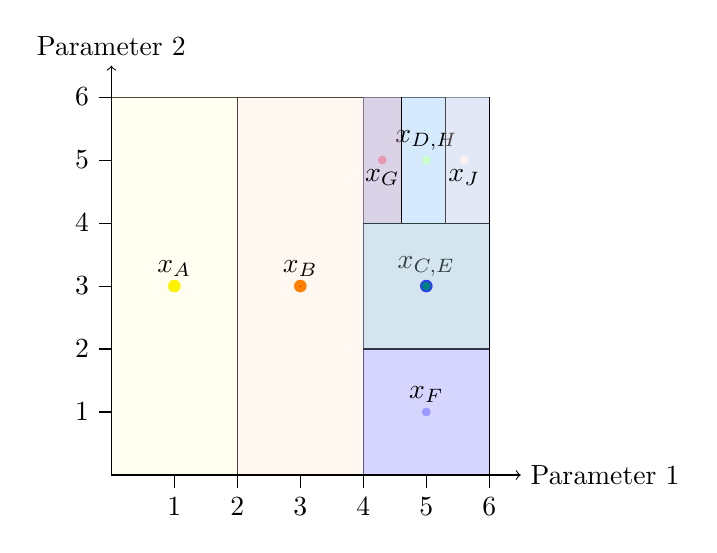
\begin{tikzpicture}[scale=0.8]

    % Define the grid
    \draw[step=6,black,very thin] (0,0) grid (6,6);

    
    % first decomposition
    \draw (2,0) -- (2,6) ;
    \draw (4,0) -- (4,6);
        % point A
        \fill[yellow!20, opacity = 0.3] (0.0,0) rectangle (2,6);
        \fill[fill = yellow] (1,3) circle (0.1) node[above]{$x_A$};  % Point in the first square
        
        % point B
        \fill[orange!20, opacity = 0.3] (2,0) rectangle (4,6);
        \fill[fill = orange] (3,3) circle (0.1) node[above]{$x_B$};  % Point in the first square
        % point C
        \fill[blue!20, opacity = 0.3] (4,0) rectangle (6,6);
        \fill[fill = blue] (5,3) circle (0.1) node[above]{$x_{C,E}$};  % Point in the first square

    % second decomposition
    \draw (4,2) -- (6,2);
    \draw (4,4) -- (6,4);
      % point D
      \fill[cyan!40, opacity = 0.3] (4,4) rectangle (6,6);
      \fill[fill = cyan!40] (5,5) circle (0.07) node[above]{$x_{D,H}$} ;  % Point in the first square
      %point E
      \fill[teal!40, opacity = 0.3] (4,2) rectangle (6,4);
      \fill[fill = teal] (5,3) circle (0.07) ;  % Point in the first square
      %point F
      \fill[blue!40, opacity = 0.3] (4,0) rectangle (6,2);
      \fill[fill = blue!40] (5,1) circle (0.07) node[above]{$x_F$} ;  % Point in the first square

    % second decomposition
    \draw (4.6,4) -- (4.6,6);
    \draw (5.3,4) -- (5.3,6);
      %point G
      \fill[purple!40, opacity = 0.3] (4,4) rectangle (4.6,6);
      \fill[fill = purple!40] (4.3,5) circle (0.07) node[below]{$x_G$} ;  % Point in the first square
      %point H
      %\fill[green!40, opacity = 0.3] (4.6,4) rectangle (5.3,6);
      \fill[fill = green!20] (5,5) circle (0.07);  % Point in the first square
      %point J
      \fill[pink!40, opacity = 0.3] (5.3,4) rectangle (6,6);
      \fill[fill = pink!20] (5.6,5) circle (0.07) node[below]{$x_J$} ;  % Point in the first square
    

    % Draw red points
    \fill[red] (3,3) circle (0.01);  % Point in the first square

    
    % Draw the axes
    \draw[->] (0,0) -- (6.5,0) node[right] {Parameter 1};
    \draw[->] (0,0) -- (0,6.5) node[above] {Parameter 2};
    
    % Add ticks and labels
    \foreach \x in {1,2,3,4,5,6} {
      \draw (\x,0) -- (\x,-0.2) node[below] {\x};
      \draw (0,\x) -- (-0.2,\x) node[left] {\x};
    }
    
\end{tikzpicture}
                }
                \caption{SOO Partition}
            \end{figure}
        \end{column}

        \begin{column}[b]{0.33\textwidth}
            \begin{figure}[h]
                \centering
                \resizebox{\textwidth}{!}{
                    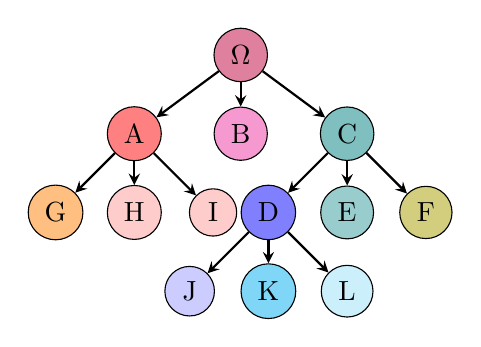
\begin{tikzpicture}[]
    \tikzstyle{space} = [circle, minimum width=0.6cm,text centered, draw=black]
    \tikzstyle{arrow} = [thick,->,>=stealth]

      \node(space)[space, fill = purple!50]{$\Omega$};


 
        %depth 1
        \node(B)[space, fill = magenta!40, below of = space, yshift = -0cm]{B};
        \node(A)[space, fill = red!50, left of = B, xshift = -10pt]{A};
        \node(C)[space, fill = teal!50,  right of = B, xshift = 10pt]{C};
        \draw[arrow] (space) -- (A);
        \draw[arrow] (space) -- (B);
        \draw[arrow] (space) -- (C);
    
    \onslide<2->{ % First loop
    %depth 1
    \node(E)[space, fill = teal!40, below of = C, yshift = -0cm]{E};
    \node(D)[space, fill = blue!50, left of = E]{D};
    \node(F)[space, fill = olive!40,  right of = E]{F};
    \draw[arrow] (C) -- (E);
    \draw[arrow] (C) -- (D);
    \draw[arrow] (C) -- (F);
    }

    \onslide<3->{
    %depth 2
    \node(H)[space, fill = red!20, below of = A]{H};
    \node(G)[space, fill = orange!50, left of = H]{G};
    \node(I)[space, fill = pink!80,  right of = H]{I};
    \draw[arrow] (A) -- (G);
    \draw[arrow] (A) -- (H);
    \draw[arrow] (A) -- (I);

    \node(K)[space, fill = cyan!50, below of = D]{K};
    \node(J)[space, fill = blue!20, left of = K]{J};
    \node(L)[space, fill = cyan!20,  right of = K]{L};
    \draw[arrow] (D) -- (J);
    \draw[arrow] (D) -- (K);
    \draw[arrow] (D) -- (L);
    }
    
    

\end{tikzpicture}
                }
                \caption{SOO Tree}
            \end{figure}
        \end{column}
    \end{columns}
\end{frame}

%---------------------------------- BaMSOO -------------------------------
\begin{frame}{Hybridization : Bayesian Multi-Scale Optimistic Optimization (BaMSOO)}
    \begin{columns}
        \begin{column}{0.55\textwidth}
            \begin{block}{Principle\footnote[7]{Wang et al. « Bayesian Multi-Scale Optimistic Optimization ». 2014} : }
                \begin{itemize}
                    \item SOO partitionning
                    \item Use a Gaussian process to enhance the scoring
                \end{itemize}
                Objective : prevent unpromising evaluations
                
            \end{block}
            
            \begin{block}{BaMSOO Scoring $g(x)$ :}
                \begin{itemize}
                    \item \textbf{If} $UCB(x) > f^+$ : {\color{gray} // \small x has potential to beat $f^+$}
                        \begin{itemize}
                            \item $g(x) = f(x)$ {\color{gray} // \small score $x$ using $f(x)$}
                        \end{itemize}
                    \item \textbf{Else } :
                        \begin{itemize}
                            \item $g(x) = LCB(x)$ {\color{gray} // \small score $x$ using $LCB(x)$}
                        \end{itemize}


                \end{itemize}
                
            \end{block}
            
        \end{column}        
        \begin{column}{0.45\textwidth}
            \begin{figure}[h]
                \centering
                \begin{algorithm}
\caption{BamSOO}
\label{algo:bamsoo}
\begin{algorithmic}[1]
\Require\\
$\Omega$: Continuous search space \\
$f$: Objective function  \Comment{train and validate the model}\\
$K$ : number of section of the space\\
$n_{max}$ : budget of evaluation \\
$K_D$ : Kernel function\\

\State $x_{0,0} \gets center(\Omega)$ 
\State  $g_{0,0} \gets    f(x_{0,0})$
\State $\mathcal T_1 = \{x_{0,0},g_{0,0},\Omega\}$\Comment{Initiate the tree}
\State  $f^+ \gets g_{0,0}$
\State $n \gets 1$ \Comment{nodes index}
\State $t \gets 1$ \Comment{evaluation index}
\State $\mathcal D_1 = \{x_{0,0},g_{0,0}\}$ \Comment{list of evaluated points}
\\

\While{$t < n_{max}$}
    \State $\nu_{max} \gets - \infty$
    \For{$h=0 \textbf{ to } depth(\mathcal T_n)$}
        \State $j \gets \arg \max_{j \in \{j | (h,j) \in L_n\}} g_{h,j}$
        \If{$g_{h,j} > \nu_{max}$}
            \State $\Omega_{h+1,j+1},\dots,\Omega_{h+1,j+K} \gets section(\Omega_{h,j},K)$
            \For{$i=1$ \textbf{to }$K$}
                \State $\mu,\sigma \gets GP(\mathcal D_t,K_D)$
                \State $N \gets N+1$
                \State $x_{h+1,j+i} \gets center(\Omega_{n})$

                \If{$\mathcal{UCB}(x_{h+1,j+i},\mu,\sigma) \geq f^+$}
                    \State $g_{h+1,j+i} \gets f(x_{h+1,j+i}) $
                    \State $t \gets t+1$
                \Else
                    \State $g_{h+1,j+i} \gets \mathcal{LCB}(x_{h+1,j+i},\mu,\sigma) $
                \EndIf

                \If{$g_{h+1,j+i} > f^+$}
                    \State $f^+ \gets g_{h+1,j+i} $
                \EndIf         
                \State $n \gets n+1$               
                \State $\mathcal T_n \gets \{(x_{h+1,j+i},f_{h+1,j+i},\Omega_{h+1,j+i})\}$  
            \EndFor  
            \State $\nu_{max} \gets g_{h,j}$
        \EndIf
    \EndFor
\EndWhile\\
\Return best of $x_{h,j},g(x_{h,j})$
\end{algorithmic}
\end{algorithm}
                \caption{Illustration of BaMSOO Algorithm}
            \end{figure}
        \end{column}
    \end{columns}
\end{frame}

%---------------------------------- Evaluation Function -------------------------------
\begin{frame}{Evaluate the solution}
    Use LitGPT framework with it's CLI to perform an evaluation of a solution. All models and datasets are taken from HuggingFace Hub.


    \begin{columns}
        \begin{column}[t]{0.45\textwidth}
            \begin{block}{Training}
                \begin{itemize}
                    \item Model : Llama-3.2-1B\footnote[2]{Touvron et al. « LLaMA: Open and Efficient Foundation Language Models »,2023}
                    \item dataset : Alpaca\footnote[3]{Hashimoto et al. « Stanford Alpaca: An Instruction-following LLaMA model ». 2024}
                    \item 1 epochs of training
                    \item Fully Sharded Data Parallelism (FSDP) as distributed strategy
                \end{itemize}
            \end{block}
        \end{column}
        \begin{column}[t]{0.45\textwidth}
            \begin{block}{Evaluating}
                Based on lm\_eval library
                \begin{itemize}
                    \item validation dataset : Hellaswag\footnote[4]{Zellers et al. « HellaSwag: Can a Machine Really Finish Your Sentence? » 2019.
                    }
                    \item testing dataset : MMLU\footnote[5]{Hendrycks et al. « Measuring Massive Multitask Language Understanding ». 2021
                    }
                \end{itemize}
            \end{block}
        \end{column}
    \end{columns}

    
\end{frame}